\documentclass[../main.tex]{subfiles}
\graphicspath{{\subfix{../img/}}}
\begin{document}
	\subsection{Machine Learning and Data}
	Il machine learning è un tipo di intelligenza artificiale che permette al sistema del computer di migliorare automaticamente le performance su una task, imparando da dati ed esempi, senza essere programmato esplicitamente per ogni azione.\\\\
	Involve lo sviluppo di algoritmi e modelli statistici che permettono al computer di imparare modelli e fare predizioni o decisioni basate sui dati in input.\\\\
	\begin{tabular}{|p{2cm}|p{6cm}|p{7cm}|}
		\hline
		\textbf{Concetto} & \textbf{Definizione} & \textbf{Caratteristiche} \\
		\hline
		\textbf{Intelligenza Artificiale} &
		Un ampio campo di studio che si concentra sulla creazione di macchine intelligenti in grado di eseguire compiti che normalmente richiedono l'intelligenza umana, come il riconoscimento vocale, la presa di decisioni e la risoluzione di problemi. &
		\begin{itemize}
			\item Risolve problemi complessi attraverso ragionamento e decisioni simili a quelli umani.
			\item Include una vasta gamma di sotto-discipline, tra cui il machine learning e il deep learning.
			\item Può essere basata su regole o guidata dai dati.
			\item Può essere applicata in numerosi settori e ambiti.
		\end{itemize}\\
		\hline
		\textbf{Machine Learning} &
		Un sottoinsieme dell'intelligenza artificiale che prevede lo sviluppo di algoritmi e modelli statistici che permettono ai computer di apprendere dai dati e fare previsioni o prendere decisioni senza essere esplicitamente programmati per ogni situazione. &
		\begin{itemize}
			\item Si concentra sulla progettazione di algoritmi che migliorano le proprie prestazioni nel tempo apprendendo dai dati.
			\item Può essere supervisionato, non supervisionato, semi-supervisionato o basato sul reinforcement learning.
			\item Può essere utilizzato per problemi di regressione e classificazione.
			\item È una componente chiave del deep learning.
		\end{itemize}
		\\
		\hline
		\textbf{Deep Learning} &
		Un sottoinsieme del machine learning che prevede l'addestramento di reti neurali artificiali su grandi quantità di dati per eseguire compiti complessi come il riconoscimento di immagini e del parlato. &
		\begin{itemize}
			\item Utilizza reti neurali artificiali con più strati per apprendere e prendere decisioni.
			\item Si concentra sullo sviluppo di reti neurali profonde con molti strati per modellare relazioni complesse nei dati.
			\item Può essere supervisionato, non supervisionato o semi-supervisionato.
			\item Utilizza grandi quantità di dati per addestrare le reti.
		\end{itemize}
		\\
		\hline
	\end{tabular}
	\subsubsection{Possibili applicazioni del ML}
	\begin{itemize}
		\item Riconoscimento di immagini e discorsi
		\item Predizione del traffico
		\item Raccomandazione di prodotti
		\item Veicoli automatici
		\item Filtro spam
		\item Riconoscimento frodi
		\item Lingua tradotta automaticamente
	\end{itemize}
	\subsubsection{ML come un processo di analisi dati}
	\begin{center}
		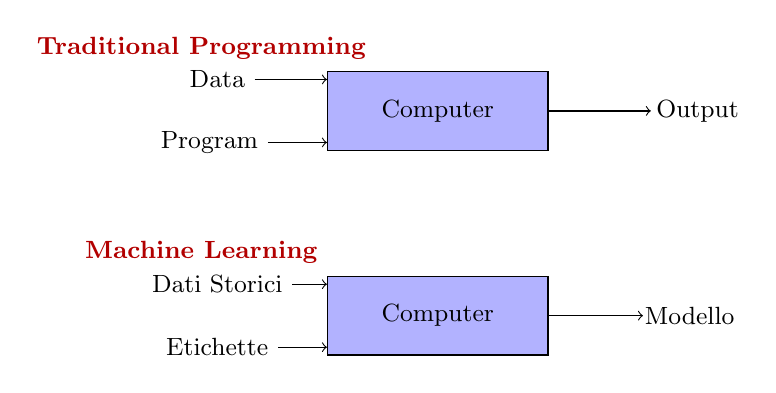
\begin{tikzpicture}[
			node distance=1cm and 2cm,
			every node/.style={font=\small},
			box/.style={draw, fill=blue!30, minimum width=2.8cm, minimum height=1cm, align=center}
			]
			
			% Traditional Programming
			\node at (0,4.8) {\textcolor{red!70!black}{\textbf{Traditional Programming}}};
			\node (prog_box) [box] at (3,4) {Computer};
			\node (data) at (0.2,4.4) {Data};
			\node (program) at (0.1,3.6) {Program};
			\draw[->] (data.east) -- (prog_box.west|-data.east);
			\draw[->] (program.east) -- (prog_box.west|-program.east);
			\node at (6.3,4) {Output};
			\draw[->] (prog_box.east) -- +(1.3,0);
			
			% Machine Learning
			\node at (0,2.2) {\textcolor{red!70!black}{\textbf{Machine Learning}}};
			\node (ml_box) [box] at (3,1.4) {Computer};
			\node (data2) at (0.2,1.8) {Dati Storici};
			\node (labels) at (0.2,1.0) {Etichette};
			\draw[->] (data2.east) -- (ml_box.west|-data2.east);
			\draw[->] (labels.east) -- (ml_box.west|-labels.east);
			\node at (6.2,1.4) {Modello};
			\draw[->] (ml_box.east) -- +(1.2,0);
		\end{tikzpicture}
	\end{center}
	\begin{center}
		\begin{tikzpicture}[
			node distance=1.5cm and 1.2cm,
			process/.style={draw, thick, minimum width=3.2cm, minimum height=1.2cm, align=center, text width=3cm},
			arrow/.style={-{Stealth}, thick},
			]
			
			% Nodes
			\node[process, fill=yellow!40] (pre) {Data\\Pre-Processing};
			\node[process, fill=blue!20, right=of pre] (train) {Model\\Training};
			\node[process, fill=green!30, right=of train] (eval) {Model\\Evaluation/Scoring};
			\node[process, fill=red!30, right=of eval] (deploy) {Model\\Deployment};
			
			% Arrows between boxes
			\draw[arrow] (pre) -- (train);
			\draw[arrow] (train) -- (eval);
			\draw[arrow] (eval) -- (deploy);
			
			% Annotations
			\draw[arrow] (train.south) ++(0,-0.3) -- ++(0,-0.7) node[below, align=center] {Estrarre un modello matematico\\(cioè l'algoritmo)};
			\draw[arrow] (eval.north) ++(0,0.3) -- ++(0,0.7) node[above, align=center] {Capire l’efficacia del modello};
			\draw[arrow] (deploy.north west) ++(0.9,0.9) node[above right] {Installazione del modello} -- (deploy.north west);
			
		\end{tikzpicture}
	\end{center}
	\begin{figure}[h]
		\centering
		\adjustbox{cfbox=white 5pt 0cm}{\includegraphics[scale=0.3]{example-image-golden}}
		\caption{Analisi dei dati tramite ML}
		\label{fig:im-30}
	\end{figure}
	\subsubsection{Dove troviamo questa metodologia: Data science}
	E' la disciplina che studia il processo di analisi dei dati. Necessitiamo di questo approccio perché abbiamo a disposizione il mondo dei big data.
	\begin{figure}[h]
		\centering
		\adjustbox{cfbox=white 5pt 0cm}{\includegraphics[scale=0.3]{example-image-golden}}
		\caption{Grafico Data Explosion}
		\label{fig:im-31}
	\end{figure}
	\begin{figure}[h]
		\centering
		\adjustbox{cfbox=white 5pt 0cm}{\includegraphics[scale=0.3]{example-image-golden}}
		\caption{Big Data and DL}
		\label{fig:im-32}
	\end{figure}
	\subsection{L’approccio data-driven, l’analisi dei dati e dei modelli predittivi}
	Modellare il mondo tramite un processo di analisi dei dati:
	\begin{itemize}
		\item Dai dati che vengono dal mondo reale;
		\item Alla definizione di un sistema guidato dai dati per il supporto alla decisione.
	\end{itemize}
	\subsubsection{Perché abbiamo bisogno di una metodologia scientifica per l’analisi dei dati}
	\textbf{Nell’approccio subsimbolico i dati sono essenziali.} \\
	La conoscenza viene appresa tramite essi
	\begin{itemize}
		\item Si trovano pattern ricorrenti e correlazioni nei dati e questo serve all'agente per classificare la situazione nuova che sta vedendo
	\end{itemize}
	Il paradigma prevalente dell’analisi dei dati parte dal presupposto che:
	\begin{itemize}
		\item I dati sono il punto di partenza di ogni analisi
		\item E’ possibile ottenere l’oggettività nei nostri modelli sul mondo collezionando dati in modo imparziale
		\item I dati parlano, cioè guidano la nostra mente nella costruzione dei modelli
	\end{itemize}
	\textbf{I dati non sono imparziali}
	\begin{itemize}
		\item Si collezionano i dati rilevanti per il problema e questo può essere collegato al tipo di soluzione/narrazione che vogliamo dare al problema
	\end{itemize}
	\textbf{I dati non sono necessariamente sufficienti}
	\begin{itemize}
		\item Non solo siamo guidati silenziosamente dalle nostre congetture nella selezione dei dati, ma se proviamo a sopprimere nozioni o schemi esplicativi, non abbiamo modo di sapere se i dati che abbiamo raccolto sono quelli più rilevanti per comprendere o risolvere i problemi in questione
		\item Non abbiamo alcun meccanismo per motivare la ricerca di ulteriori dati che possano fornire conferme, confutazioni o ulteriori approfondimenti
	\end{itemize}
	\textbf{I dati non parlano, tanto meno spiegano}
	\begin{itemize}
		\item Non si è a conoscenza di un processo oggettivo e deduttivo che da una mole di dati generi una teoria. Quindi i dati non parlano
		\item Non si può nemmeno interpretare i dati senza ricorrere a un contesto teorico
	\end{itemize}
	\textbf{Il problema:} \\
	Le informazioni che cercheremo e troveremo ci basteranno, non vedendo cosa possa essere pericoloso. \\
	Quindi i dati motivano le congetture, il tentativo ci permette di distinguere le ipotesi e guidarci per la selezione dei dati, motivando la ricerca e la scoperta di essi.
	\subsection{Data Science e una metodologia per l’analisi dei dati}
	\subsubsection{Data Science}
	E’ l’insieme di principi metodologici (basati sul metodo scientifico) e tecniche multidisciplinari volto a interpretare ed estrarre conoscenza dai dati attraverso la relativa fase di analisi da parte di un esperto.
	\subsubsection{I cinque passi della Data Science}
	I cinque passi fondamentali per la scienza dei dati sono i seguenti:
	\begin{enumerate}
		\item Porre una domanda interessante
		\item Ottenere i dati
		\item Esplorare i dati
		\item Creare un modello per i dati
		\item Comunicare e presentare i risultati
	\end{enumerate}
	I punti 2, 3, 4 e 5 sono i passi più tecnici di un processo di scienza dei dati.
	\subsection{Data Science - Modelli predittivi}
	\subsubsection{Trovarle correlazioni fra i dati}
	I coefficienti di correlazione sono una misura quantitativa che descrive l’intensità dell’associazione/relazione fra due variabili (compresa tra -1 e 1).\\\\
	La correlazione fra due insiemi di dati ci dice quanto si “muovono insieme”. \\
	Gli algoritmi di Machine Learning cercano e sfruttano queste relazioni tra i dati per offrire previsioni accurate.\\\\
	In generale, una correlazione tenterà di misurare una relazione lineare fra le variabili.
	\begin{itemize}
		\item Una correlazione positiva significa che quando una variabile aumenta, anche l’altra tende ad aumentare
		\item Una correlazione negativa significa che quando una variabile aumenta, l’altra tende a diminuire
		\item Minima correlazione è a 0
	\end{itemize}
	Se non viene individuata una correlazione in questo modo, ciò non significa che non esiste alcuna relazione fra le variabili, ma solo che non esiste una linea “best fit” per le linee.\\\\
	Quando i grafici e le statistiche mentono, in realtà mentono le persone. \\
	Uno dei modi più facili per ingannare consiste nel \textbf{confondere la correlazione e la causalità}.
	\begin{itemize}
		\item La correlazione è una metrica quantitativa compresa fra -1 e 1 che misura come si spostano due variabili l’una rispetto all'altra e stabilisce il grado con il quale le variabili cambiano insieme;
		\item La causalità è l’idea che una variabile influenzi un’altra e determini effettivamente il valore di un’altra.
	\end{itemize}
	Molto spesso capita che due variabili siano, si, correlate, ma senza alcuna relazione di causalità fra di esse. \\
	Potrebbe entrare in gioco un fattore di confusione.\\\\
	\textbf{Fattore di confusione}: Esiste “in agguato” una terza variabile non individuata e che funge da collegamento fra le due variabili.\\\\
	Correlazione o causalità? In alcuni casi le variabili potrebbero non avere proprio nulla a che fare l’una con l’altra! Il tutto potrebbe essere semplicemente frutto di coincidenza. \\
	Vi sono molte variabili che sono correlate ma senza alcuna relazione di causalità.\\\\
	\textbf{Attenzione al paradosso di Simpson} \\
	Il paradosso stabilisce che una correlazione fra due variabili può essere completamente invertita considerando fattori differenti. \\
	Questo significa che anche se un grafico potrebbe mostrare una correlazione positiva, queste variabili possono diventare anti-correlate prendendo in considerazione un altro fattore.
	\paragraph{Esempio}
	Il consumo di mozzarella determina il numero di lauree in ingegneria civile a livello mondiale.\\
	I due andamenti sono molto simili, eppure non esiste un legame causale tra essi.
	\begin{figure}[h]
		\centering
		\adjustbox{cfbox=white 5pt 0cm}{\includegraphics[scale=0.3]{example-image-golden}}
		\caption{Mozzarella consumption graph}
		\label{fig:im-33}
	\end{figure}
	\\{\color{red} Esempio nel pacco di slide "Intro\_IA-32-Modelli Predittivi" a pagine 37, 38, 39}
	\subsection{Machine learning}
	\subsubsection{Che cosa si intende con machine learning?}
	Dare ai computer la capacità delle macchine di apprendere dai dati, senza ricevere regole esplicite da un programmatore. \\
	Il machine learning si occupa della capacità di trarre dai dati determinati pattern (segni), anche se i dati contengono errori (rumore).\\\\
	In machine learning, al modello non viene detto qual è la soluzione migliore; piuttosto riceve vari esempi del problema e gli viene chiesto di decidere qual è la soluzione migliore.
	\subsubsection{ML (algoritmi predittivi) vs algoritmi classici}
	Riconoscimento di un volto: 
	\begin{itemize}
		\item Classico 
		\begin{itemize}
			\item Nell’algoritmo viene inserito un codice che definisce un volto come una forma tondeggiante, con due occhi, capelli, naso e così via
			\item L’algoritmo ricercherà nella fotografia queste caratteristiche “cablate” e dirà se è stato in grado o meno di trovarle 
		\end{itemize}
		\item Predittivo
		\begin{itemize}
			\item Non viene mai detto che cos’è un volto: vengono solo forniti degli esempi (training set), alcuni con volti, altri senza
			\item Il compito del modello di machine learning è trovare la differenza. \\
			Una volta individuata la differenza, usa queste informazioni per accettare una nuova immagine e predire se contiene o meno un volto.
		\end{itemize}
	\end{itemize}
	\subsubsection{Il machine learning non è perfetto} 
	Quasi nessun modello di machine learning tollera l’impiego di dati “sporchi”, con valori mancanti o valori categorici. 
	\begin{itemize}
		\item I dati usati sono già stati pre-elaborati e ripuliti.
	\end{itemize}
	Ogni riga di un dataset ripulito rappresenta una singola osservazione dell’ambiente che stiamo tentando di modellare. 
	\begin{itemize}
		\item Se l’obiettivo è quello di trovare le relazioni esistenti fra le variabili, allora si deve partire dal presupposto che fra queste variabili esista in effetti una relazione.
	\end{itemize}
	Gli algoritmi non sono in grado di comunicare che tale relazione, in realtà, non esiste.\\\\
	La macchina è molto abile, ma fatica a collocare le cose nel loro contesto: 
	\begin{itemize}
		\item L’output è una serie di numeri e metriche che tentano di quantificare l’efficacia del modello
		\item Compito dell’essere umano valutare queste metriche e comunicare i risultati
	\end{itemize}
	La maggior parte dei modelli di machine learning è sensibile alla rumorosità dei dati. 
	\begin{itemize}
		\item Questo significa che i modelli si confondono quando si includono dati insensati.
	\end{itemize}
	\subsection{Algoritmi predittivi}
	\subsubsection{Tipi di ML (algoritmi predittivi)}
	La scelta dell’algoritmo:
	\begin{itemize}
		\item Ha impatto sulle modalità di preparazione dei dati
		\item Comporta una susseguente attività di sistemazione dati
	\end{itemize}
	Si possono classificare per:
	\begin{itemize}
		\item Scopo
		\item Caratteristiche delle modalità di apprendimento e tecniche utilizzate:
		\begin{itemize}
			\item Tipi di dati/strutture organiche utilizzati (albero/grafo/rete neurale)
			\item Campo della matematica dal quale attinge maggiormente (statistica/calcolo delle probabilità)
			\item Livello di calcolo richiesto per l’addestramento (apprendimento profondo - deep learning)
		\end{itemize}
	\end{itemize}
	\subsubsection{Classificazione degli algoritmi per scopo}
	Permette di identificare quali algoritmi siano adatti ad un particolare problema predittivo
	\begin{itemize}
		\item Classificazione
		\item Regressione
		\item Clustering
		\item Association rules
		\item Serie temporali
	\end{itemize}
	\paragraph{Classificazione} 
	Individuazione dell’appartenenza di un elemento ad una classe.\\
	L’output della classificazione è categorico e quindi può assumere un numero finito di possibili valori. \\
	Agli algoritmi di classificazione appartengono i classificatori lineari, gli alberi decisionali e le reti neurali.
	\begin{figure}[h]
		\centering
		\adjustbox{cfbox=white 5pt 0cm}{\includegraphics[scale=0.3]{example-image-golden}}
		\caption{Classificazione}
		\label{fig:im-34}
	\end{figure}
	\paragraph{Regressione} 
	L’output del modello è un valore numerico, che si vuole approssimare tramite una funzione dei dati di input. \\
	La variabile di output è continua e può assumere un numero infinito di valori.\\
	Algoritmi che appartengono a questa categoria sono: la regressione lineare.
	\begin{figure}[h]
		\centering
		\adjustbox{cfbox=white 5pt 0cm}{\includegraphics[scale=0.3]{example-image-golden}}
		\caption{Regressione}
		\label{fig:im-35}
	\end{figure}
	\paragraph{Clustering} 
	Il raggruppamento degli elementi di un dataset in gruppi (i cluster) utilizzando soltanto le informazioni contenute nei dati di input (apprendimento non supervisionato). \\
	L'output del clustering (ovvero la categorizzazione) non è noto a priori. I raggruppamenti sono realizzati in base alla similarità dei punti.\\
	Es. clustering: k-means.
	\subsubsection{Classificazione per modalità di apprendimento} 
	Il procedimento con cui l'algoritmo impara dai dati di input è chiamato training.
	\begin{itemize}
		\item Supervisionato
		\item Non supervisionato
		\item Semi-supervisionato
	\end{itemize}
	\paragraph{Supervisionato} 
	Modelli di analisi predittiva $\Rightarrow$ capacità di prevedere il futuro sulla base del passato. \\
	Il machine learning con supervisione richiede l'impiego di un determinato tipo di dati: i dati etichettati.\\\\
	L'apprendimento con supervisione funziona usando delle parti dei dati per prevedere un’altra parte. \\
	Si devono separare i dati in due parti:
	\begin{enumerate}
		\item I \textbf{predittori}, che sono le colonne che verranno usate per effettuare la previsione. 
		\begin{enumerate}
			\item Sono chiamate anche caratteristiche, input, variabili o variabili indipendenti.
		\end{enumerate}
		\item La \textbf{risposta}, che è la colonna che vogliamo prevedere. 
		\begin{enumerate}
			\item Questo è chiamato anche risultato, etichetta, target e variabile dipendente.
		\end{enumerate}
	\end{enumerate}
	L'apprendimento con supervisione tenta di trovare una relazione fra i predittori e la risposta per effettuare una previsione. \\
	Questa relazione rappresenta una regola generale di classificazione detta modello. \\
	Una volta costruito il modello, la macchina lo utilizza per classificare le nuove istanze.
	\paragraph{Non supervisionato} 
	Non tentano di trovare una relazione fra i predittori e una specifica risposta e pertanto non vengono usati per effettuare previsioni di alcun tipo. \\
	Al contrario, vengono utilizzati per trovare nei dati forme di organizzazione e di rappresentazione precedentemente sconosciute. \\
	Possono ridurre le dimensioni dei dati condensando insieme più variabili. \\
	Trovare dei gruppi di osservazioni che si comportano allo stesso modo e raggrupparli (clustering).\\\\
	\underline{Vantaggi}: Non richiede dati etichettati. \\
	\underline{Difetti}: Si perde ogni potere predittivo ed è difficile capire se si comporta correttamente
	\paragraph{Semi-supervisionato} 
	Lavorano su un insieme di dati che solo in parte possiede già una classificazione. \\
	Solitamente, la parte di dati già classificata è una piccola percentuale del dataset, ma è sufficiente a rendere l'algoritmo più preciso. \\
	Utile quando vi è grande disponibilità di dati non classificati ed il costo per classificarli manualmente è molto alto.
	\subsection{Costruire un modello di ML}
	\subsubsection{Programmazione classica e ML}
	Nella programmazione classica dato un problema e un certo insieme di dati di input, il programmatore realizza un algoritmo che produce un certo risultato (un insieme di dati di output). \\
	Se non cambia il problema, l'algoritmo è lo stesso per qualunque configurazione dei dati. \\
	L'output è il risultato dell'applicazione dell'algoritmo ai dati.\\\\
	Nel Machine Learning dato un problema e un certo insieme di dati di input, viene fornita un'esperienza (sotto forma di soluzioni desiderate o reazioni dell'ambiente alla macchina). \\
	Sulla base di questi fattori, il metodo di ML costruisce un modello di algoritmo che si adatta ai dati. \\
	L'output è l'algoritmo, cioè il risultato dell'apprendimento della macchina.
	\subsubsection{Gli algoritmi di ML}
	\textbf{Modello di ML vs Algoritmo}
	\begin{itemize}
		\item Un algoritmo è una sequenza di istruzioni logicamente organizzate e definite che descrive un processo o una procedura computazionale
		\item Un modello è un software che viene inserito nell'algoritmo e che ci serve per trovare la soluzione al nostro problema
		\begin{itemize}
			\item Poiché spesso non conosciamo la vera soluzione, queste vengono chiamate predizioni.
		\end{itemize}
	\end{itemize}
	Un \textbf{modello addestrato} di machine learning verrà poi implementato all'interno di un algoritmo che se eseguito dalla macchina restituisce sulla base degli input l'output più corretto secondo il modello che ha al suo interno. \\
	Il modello deve essere addestrato in una fase precedente.\\\\
	Un modello addestrato di ML è un file che è il risultato di un programma in grado modificare alcuni parametri del modello sulla base di dati di training. \\
	Costruire un modello nell'apprendimento automatico significa creare una rappresentazione matematica generalizzando e imparando dai dati di addestramento.\\\\
	Un algoritmo di machine learning è un metodo matematico per individuare schemi ricorrenti in un set di dati. \\
	Gli algoritmi di machine learning sono spesso ricavati da statistiche, calcolo e algebra lineare.\\\\
	Il \textbf{processo di esecuzione} di un algoritmo di machine learning su un set di dati (chiamati dati di addestramento) e l'ottimizzazione dell'algoritmo per la ricerca di determinati schemi o risultati viene detto addestramento del modello.\\\\
	I \textbf{parametri del modello} sono variabili interne del modello di ML che vengono appresi e stimati durante l'addestramento dal set di dati.\\\\
	La \textbf{funzione risultante} (memorizzata in un file/software) con regole e strutture di dati viene chiamata \textbf{modello addestrato} di machine learning.
	\paragraph{Implementazione del modello di machine learning} 
	L'implementazione è il processo con cui un modello di machine learning viene reso disponibile per l'utilizzo in un ambiente di destinazione. \\
	Il linguaggio più utilizzato è Python e la libreria più famosa Scikit-learn.
	\subsection{Problematiche comuni agli algoritmi di ML}
	{\color{red}Approfondimento su slide "Intro\_IA-32-Modelli Predittivi" pagine 75-84}
	\subsubsection{Hyperparameter tuning}
	\subsubsection{Grid Search (o parameter sweep)}
	\subsubsection{Random Search}
	\subsubsection{Overfitting}
	Accade quando un modello è troppo complesso ed eccessivamente adattato ai dati di training. \\
	La crescita della complessità del modello diminuisce l’errore predittivo sui dati del training set.\\\\
	Un modello sovradimensionato è un modello matematico che contiene più parametri di quelli che possono essere giustificati dai dati.\\\\
	All'aumentare della complessità del modello diminuisce anche l’errore sul test set, ma solo fino ad un certo punto:
	\begin{itemize}
		\item L’errore infatti ritorna a crescere superata una certa soglia di complessità
		\item La crescita di questo errore segnala che si sta entrando nel territorio dell’overfitting
	\end{itemize}
	3 termini importanti:
	\begin{itemize}
	\item \textbf{Bias}: Rappresenta quanto, in media, le previsioni di un modello sono lontane dalla realtà
	\item \textbf{Varianza}: Indica di quanto le stime variano attorno alla media
	\item \textbf{Underfitting}: In questo caso il modello è troppo semplice per poter avere in media una buona performance predittiva
	\end{itemize}
	\subsubsection{Utilizzo di un approccio addestramento/test}
	\paragraph{Capacità di generalizzazione}
	\subsection{Basic algorithms in machine learning}
	\subsubsection{Algoritmi di classificazione}
	La classificazione individua l'appartenenza ad una classe. \\
	Cerca di predire (restituire) l'uscita più probabile dando in ingresso un numero limitato di input (predittori, caratteristiche /features) l'uscita (l'etichetta).
	\subsubsection{Classificazione}
	A partire da un fenomeno l'esperto di ML ne esegue l'analisi e individua le sue principali caratteristiche o features. \\
	Queste features sono organizzate in osservazioni o cases e corrispondenti ai valori target o labels. \\
	A questo punto la macchina si “addestra” ( fase di training) a riconoscere quali valori delle features producono certi target (si dice che riconosce dei pattern nei dati) e costruisce un modello che si adatta ai target richiesti. \\
	Terminata la fase di addestramento, il modello è pronto per avere in input nuove osservazioni e prevedere quale potrebbe essere il valore target di uscita, corredato di una valutazione della bontà della previsione.
	\subsubsection{Classificatore Naive (ingenuo) Bayes}
	Il Naive Bayes è un algoritmo classificatore probabilistico basato sul teorema di Bayes. \\
	Calcola la probabilità di ogni etichetta per un determinato oggetto osservando le sue caratteristiche. \\
	Poi, sceglie l'etichetta con la probabilità maggiore. \\
	Per usare il classificatore bayesiano occorre conoscere o stimare le probabilità a priori e condizionali del problema.\\\\
	Cosa fa il teorema di Bayes:
	\begin{itemize}
		\item Si supponga di voler classificare della frutta (si faccia finta che siano solo due per semplificare la spiegazione) che viene mostrata a un osservatore
		\item Per gli esseri umani, ma allo stesso modo deve essere fatto per le macchine, determinare la tipologia di frutta che si sta osservando, avviene esaminando determinate caratteristiche (feature) estratte dall'osservazione della frutta, attraverso opportune tecniche
		\item Parte dal presupposto dell'indipendenza fra le variabili e usa le probabilità per classificare gli oggetti in base alle loro caratteristiche
		\item La teoria bayesiana di decisione svolge un ruolo importante solo quando risultano conosciute alcune informazioni a priori sugli oggetti.
	\end{itemize}
	Il Naive Bayes parte dal presupposto dell'indipendenza fra le variabili e usa le probabilità per classificare gli oggetti in base alle loro caratteristiche.\\
	{\color{red}Approfondimento su slide "Intro\_IA-32-Modelli Predittivi" pagine 91-110}
	\paragraph{Esempio} 
	Un frutto può essere classificato nella classe "mele" se è di colore rosso, ha un diametro di circa 10 cm e ha una forma rotonda. \\
	Sono tre caratteristiche differenti. \\
	Un algoritmo di Naive Bayes classifier considera ognuna di queste caratteristiche come un contributo indipendente alla probabilità complessiva che il frutto sia una mela. \\
	Non considera le possibili correlazioni tra le caratteristiche.
	\subsubsection{La probabilità condizionata e il teorema di Bayes}
	Dati due eventi $A$ e $B$, si definisce probabilità condizionata $P(A \vert B)$ la probabilità del verificarsi dell'evento $A$, condizionata al fatto che sia verificato l'evento $B$: $P(A \vert B)=P(A \cap B)/P(B)$.\\\\
	Il Teorema di Bayes si ricava mettendo in rapporto $P(A \vert B)=P(A \cap B)/P(B)$ e $P(B \vert A)=P(A \cap B)/P(A)$ ottenendo $P(A \vert B)=P(B \vert A) \cdot P(A)/P(B)$.\\\\
	Questo ci permette di esprimere la probabilità a posteriori $P(A \vert B)$ che una determinata ipotesi $A$ sia verificata in presenza del verificarsi di una evidenza $B$.\\
	{\color{red}Approfondimento su slide "Intro\_IA-32-Modelli Predittivi" pagine 91-110}
	\subsubsection{Classificatore di bayes vantaggi e svantaggi}
	Vantaggi: 
	\begin{itemize}
		\item Utilizzo semplice e facilmente intuibile il funzionamento
		\item EFFICIENTE in termini computazionali
		\item Non ha bisogno di grandi quantità di dati
		\item Ancora oggi risolve egregiamente alcuni problemi di classificazione con discreta efficienza.
	\end{itemize}
	Svantaggi: 
	\begin{itemize}
		\item Richiede conoscenza di tutti i dati del problema
		\item L'algoritmo fornisce un'approssimazione "ingenua" (naive) del problema perché non considera la correlazione tra le caratteristiche dell'istanza.
	\end{itemize}
	{\color{red}Approfondimento su slide "Intro\_IA-32-Modelli Predittivi" pagine 91-110}
	\subsubsection{Alberi decisionali (Decision Trees)}
	Sono uno dei metodi di calcolo principalmente utilizzati nel data mining, in particolare per determinare a quale categoria appartiene un elemento, in base al valore dei suoi attributi noti.\\\\
	Un albero decisionale è una struttura a grafo che include un nodo radice, da cui partono dei rami che arrivano a dei nodi figli. \\
	I nodi terminali sono detti "nodi foglia".
	\begin{enumerate}
		\item Ogni nodo interno denota un test su un attributo
		\item Ogni ramo indica il risultato di un test
		\item Ogni nodo foglia contiene un'etichetta di classe
		\item Il nodo più in alto nell'albero è il nodo radice
	\end{enumerate}
	\begin{figure}[h]
		\centering
		\adjustbox{cfbox=white 5pt 0cm}{\includegraphics[scale=0.3]{example-image-golden}}
		\caption{Esempio albero decisionale}
		\label{fig:im-36}
	\end{figure}
	Ogni nodo interno rappresenta un test su un attributo: Weather, Time, Hungry. \\
	Ogni nodo foglia rappresenta una classe: Walk, Bus.\\
	I vantaggi di avere un albero decisionale sono i seguenti:
	\begin{itemize}
		\item Non richiede alcuna conoscenza di dominio
		\item È facile da capire
		\item Le fasi di apprendimento e classificazione di un albero decisionale sono semplici e veloci
	\end{itemize}
	L'algoritmo si fonda sul concetto di \textbf{entropia della teoria dell'informazione}.\\\\
	Ora, per ciascun attributo del nostro dataset, dobbiamo trovare quella ripartizione, basata sui valori dell'attributo, per la quale il guadagno è massimo. \\
	La ripartizione che massimizza il guadagno corrisponde al primo livello dell'albero, sotto l'insieme totale. \\
	A questo punto si ripete il processo per ciascuno dei sottoinsiemi che, al loro interno, presentano elementi appartenenti a classi diverse. \\
	Il processo si ferma quando i sottoinsiemi contengono elementi solo di una classe, oppure quando il continuare con la suddivisione non porta miglioramenti dell'accuratezza.\\\\
	Gli algoritmi degli alberi decisionali includono \textbf{tecniche di pruning} che hanno lo scopo di limitare la crescita dell'albero.\\
	Il pruning evita che l'albero decisionale si adatti troppo ai dati di training, causando l'overfitting del modello.\\\\
	Vantaggi:
	\begin{itemize}
		\item La produzione di regole come parte dell'output dell'algoritmo, consentendo una facile interpretazione dei risultati
		\item Possono gestire feature con relazioni lineari e non lineari con l'output
	\end{itemize}
	Svantaggi:
	\begin{itemize}
		\item Sono instabili, il che significa che un piccolo cambiamento nei dati può portare a un grande cambiamento nella struttura dell'albero decisionale ottimale
		\item Sono spesso relativamente imprecisi. Molti altri predittori funzionano meglio con dati simili
	\end{itemize}
	La regressione predice un valore numerico specifico.\\ Determinano il valore di una variabile continua in base alle feature di input.\\
	{\color{red}Approfondimento su slide "Intro\_IA-32-Modelli Predittivi" pagine 111-124}
	\subsubsection{Support Vector Machines}
	{\color{red}Approfondimento su slide "Intro\_IA-32-Modelli Predittivi" pagine 125-131}
	\subsubsection{Fuzzy rules based systems}
	{\color{red}Approfondimento su slide "Intro\_IA-32-Modelli Predittivi" pagine 131-136}
	\subsubsection{Algoritmi di regressione}
	\paragraph{Regressione lineare}
	\begin{itemize}
		\item Assume che la relazione tra la variabile target e le variabili di input sia lineare
		\item La relazione comprende anche una variabile di errore, ovvero una variabile casuale non rilevata, che aggiunge rumore alla relazione lineare
	\end{itemize}
	Si assume che l'errore abbia una distribuzione normale con media $0$ e varianza costante e quindi non cambi al variare dei valori delle feature di input.
	\begin{figure}[h]
		\centering
		\adjustbox{cfbox=white 5pt 0cm}{\includegraphics[scale=0.3]{example-image-golden}}
		\caption{Regressione lineare}
		\label{fig:im-37}
	\end{figure}
	Sia:
	\begin{itemize}
		\item $y$ il vettore che rappresenta la variabile target;
		\item $X$ la matrice delle feature;
		\item $\beta$ (Beta) il vettore dei parametri da stimare;
		\item $\varepsilon$ (Epsilon) variabile casuale dell'errore.
	\end{itemize}
	\[y = X \cdot \beta + \varepsilon\]
	\paragraph{Regressione logistica}
	{\color{red}Approfondimento su slide "Intro\_IA-32-Modelli Predittivi" pagine 137-141}
	\subsubsection{Algoritmi semi-supervisionati}
	{\color{red}Approfondimento su slide "Intro\_IA-32-Modelli Predittivi" pagine 142-146}
	\subsubsection{Algoritmi di clustering}
	\textbf{Tipico problema non supervisionato} \\
	E' un insieme di metodi per raggruppare oggetti in classi omogenee. \\
	Un cluster è un insieme di oggetti che presentano tra loro delle similarità, ma che presentano dissimilarità con oggetti in altri cluster. \\
	L'input di un algoritmo di clustering è costituito da un campione di elementi, l'output è dato da un certo numero di cluster in cui gli elementi del campione sono suddivisi in base a una misura di similarità.\\\\
	La cluster analysis è ampiamente utilizzata:
	\begin{itemize}
		\item Ricerche di mercato
		\item Riconoscimento di pattern
		\item Raggruppamento di clienti in base ai comportamenti d’acquisto
		\item Posizionamento dei prodotti
		\item Analisi dei social network, per il riconoscimento di community di utenti
		\item Identificazione degli outliers
	\end{itemize}
	\textbf{Outliers} \\
	La loro identificazione può essere interessante per due scopi:
	\begin{itemize}
		\item L’eliminazione di questi valori anomali, che potrebbero essere causati da errori
		\item L’isolamento di questi casi che magari rivestono una certa importanza per il business
	\end{itemize}
	\textbf{Algoritmo k-means}:
	\begin{enumerate}
		\item Definiamo il numero k di cluster desiderati
		\item Partizioniamo l’insieme in K cluster, assegnando a ciascuno di essi degli elementi scelti a caso
		\item Calcoliamo i centroidi di ciascun cluster k con la formula in alto
		\item Calcoliamo la distanza degli elementi del cluster dal centroide, ottenendo un errore quadratico, con la formula in basso
		\item A questo punto si riassegnano gli elementi del campione in base al più vicino centroide
		\item Si ripetono i passaggi 2, 3, 4 e 5 finché il valore minimo dell’errore totale non è raggiunto, oppure finché i membri dei cluster non si stabilizzano, oppure finché non si raggiunge un numero massimo di iterazioni, predefinito
	\end{enumerate}
	L'algoritmo k-means è sensibile all’allocazione iniziale dei valori e, in base ad essa, potrebbe convergere a un minimo locale della funzione d’errore e non al minimo assoluto. \\
	Sempre a causa dell’allocazione iniziale casuale, i risultati del k-means potrebbero essere diversi ad ogni esecuzione sugli stessi dati. Inoltre è molto sensibile al rumore nei dati e alla presenza di outliers.
	\subsubsection{Model ensembles}
	{\color{red}Approfondimento su slide "Intro\_IA-32-Modelli Predittivi" pagine 163-174}
	\subsubsection{Reti Neurali}
	{\color{red}Approfondimento su slide "Intro\_IA-32-Modelli Predittivi" pagine 175-201}
	\subsection{Il test e la valutazione dei modelli predittivi} 
	Le modalità di valutazione sono diverse a seconda del tipo di algoritmo:
	\begin{itemize}
		\item I modelli di classificazione
		\item I modelli di regressione
		\item I modelli di clustering (utilizzate anche nei task di regressione).
	\end{itemize}
	\subsubsection{Hold-out e cross validation} 
	Si prende un numero finito k di parti (fold) di uguali dimensioni.\\
	Per ogni subset si considera k1 delle parti come set di addestramento e la parte rimanente come set di collaudo. \\
	Quindi si calcoliamo una determinata metrica per ogni parte. \\
	Alla fine si calcola la media dei risultati.
	\begin{figure}[h]
		\centering
		\adjustbox{cfbox=white 5pt 0cm}{\includegraphics[scale=0.3]{example-image-golden}}
		\caption{Holdout Strategy}
		\label{fig:im-38}
	\end{figure}
	\begin{figure}[h]
		\centering
		\adjustbox{cfbox=white 5pt 0cm}{\includegraphics[scale=0.3]{example-image-golden}}
		\caption{K-fold Strategy}
		\label{fig:im-39}
	\end{figure}
	\subsubsection{Cross validation e matrice di confusione}
	Dalla cross validation scaturiscono metriche di valutazione che consentono di effettuare la scelta dell’algoritmo o della parametrizzazione migliore. \\
	La più utilizzata è la matrice di confusione che altro non è che una cross tabulazione delle classi reali e delle classi predette.
	\begin{figure}[h]
		\centering
		\adjustbox{cfbox=white 5pt 0cm}{\includegraphics[scale=0.3]{example-image-golden}}
		\caption{Matrice di confusione}
		\label{fig:im-40}
	\end{figure}
	\paragraph{Matrice di confusione}
	\begin{itemize}
		\item Il quadrante (1,1), che indica quanti elementi della classe positiva sono stati correttamente individuati dall'algoritmo (veri positivi o True Positive o TP).
		\item Il quadrante (0,0), che indica quanti elementi della classe negativa sono stati correttamente individuati dall'algoritmo (veri negativi o True Negative o TN).
		\item Il quadrante (0,1), che indica quanti elementi della classe negativa reale sono stati posti dall'algoritmo nella classe positiva (falsi positivi o False Positive o FP).
		\item Il quadrante (1,0), che indica quanti elementi della classe positiva reale sono stati posti dall'algoritmo nella classe negativa (falsi negativi o False Negative o FN).
	\end{itemize}
	\paragraph{Matrice di confusione e metriche di valutazione del modello}
	\begin{itemize}
		\item Accuracy: $\frac{(TP + TN)}{(P + N)}$
		\item Precision (o Positive Predictive Value): $\frac{TP}{(TP + FP)}$
		\item Sensitivity (o Recall o True Positive Rate): $\frac{TP}{(TP + FN)} = \frac{TP}{P}$
		\item Specificity (o True Negative Rate): $\frac{TN}{(TN + FP)} = \frac{TN}{N}$
	\end{itemize}
	\textbf{Attenzione}: L’accuracy è una misura che potrebbe essere fuorviante.\\\\
	Per ottimizzare l’algoritmo è bene impiegare la metrica più adeguata al problema e cioè:
	\begin{itemize}
		\item L’\textbf{accuracy} quando desideriamo che la maggior parte degli elementi siano correttamente classificati, indipendentemente dalla produzione di falsi positivi o falsi negativi.
		\item La \textbf{sensitivity} quando vogliamo massimizzare i True Positive senza però far crescere troppo i False Positive.
		\item La \textbf{precision} quando vogliamo massimizzare i veri positivi e minimizzare i falsi negativi.
		\item La \textbf{specificity} quando occorre massimizzare il numero di veri negativi.
	\end{itemize}
	\paragraph{Matrice di confusione e F-measure}
	\textbf{F-measure} è una misura dell’accuratezza di un test e si deriva dalla matrice di confusione.\\\\
	La misura tiene in considerazione precisione e recupero del test, dove la precisione è il numero di veri positivi diviso il numero di tutti i risultati positivi, mentre il recupero è il numero di veri positivi diviso il numero di tutti i test che sarebbero dovuti risultare positivi (ovvero veri positivi più falsi negativi).
	\[F \; measure = \frac{2 \cdot sensitivity \cdot precision}{sensitivity + precision} = \frac{2 \vert TP \vert}{2 \vert TP \vert + \vert FP \vert + \vert FN \vert}\]
	\subsubsection{Valutazione dei modelli di clustering}
	La misura più comunemente utilizzata è lo scarto quadratico medio (\textbf{SSE - Sum of Squared Error}). \\
	Per ogni punto l’errore è la distanza dal centroide del cluster a cui esso è assegnato
	\[SSE = \sum_{l = 1}^{K} \sum_{x \in C_i} dist^2 (m_l , x)\]
	$x$ è un punto appartenente al cluster $C_i$ e $m_i$ è il rappresentante del cluster $C_i$
	\[m_i = \sum_{x \in c_i} x\]
	Ovviamente il valore di $SSE$ si riduce incrementando il numero dei cluster $K$.
\end{document}